%************************************************
\chapter{Grounded Learning of Knowledge Utility}
\label{chapter:grounded_learning_of_knowledge_utility}
%************************************************

Hypothetical type knowledge transframes are used by the deliberative
and reflective planning machines in order to infer the effects of
executing multi-step plans.  There is a distinction here made between
the \emph{factual} knowledge that is directly an abstraction of
knowledge grounded in the physical or deliberative planning machine
knowledge bases, which are not based on any learned action hypotheses,
and the \emph{counterfactual} knowledge that is inferred and supported
by hypotheses of the effects of resource executions that the AI has
either ``been told'' or has learned in the course of actually
executing those resources in different contexts.  In order to maintain
this distinction in the AI, different knowledge bases are used to
separate the factual knowledge from counterfactual knowledge.  Factual
knowledge is induced into factual type knowledge abstractions.  The
factually grounded knowledge bases include the visual, physical,
physical type, deliberative planning machine, and deliberative
planning machine type knowledge bases.  However, the addition of
factually grounded knowledge causes a loss of hypotheses from the
resource execution type knowledge transframe hypothesis spaces in both
the deliberative and reflective layers.  Each counterfactual event in
the counterfactual knowledge bases has a list of dependencies that
must maintain their support in order for the counterfactual knowledge
to continue to exist.  Dependencies in the AI have three types of
support that a dependency can rearrange in order to maintain its
support of its dependent counterfactual knowledge events:
\begin{enumerate}
\item Future resource activation dependencies.
\item Resource execution transframe change hypothesis dependencies.
\item Resource execution transframe precondition knowledge dependencies.
\end{enumerate}
If any of these three types of supports loses its hypothetical factual
grounding, this loss of hypothetical factual grounding causes the
dependency to become \emph{invalidated}.  Once a dependency has become
invalidated, it has a chance to find new hypothetical grounding before
it becomes \emph{unsupported}.  Counterfactual event knowledge is
notified when a dependency has become unsupported, causing the
counterfactual events to be removed from the counterfactual event
knowledge bases.  Also, as some counterfactual knowledge may form
hypothetical grounding of further dependencies of further
counterfactual event knowledge, the loss of support for a dependency
can cause a chain reaction through events and their dependent
dependencies.  In this way, additional factual knowledge refines and
reduces the counterfactual knowledge that has been inferred in the
counterfactual event knowledge bases of the deliberative and
reflective layers of the AI.
\begin{figure}[h]
\centering
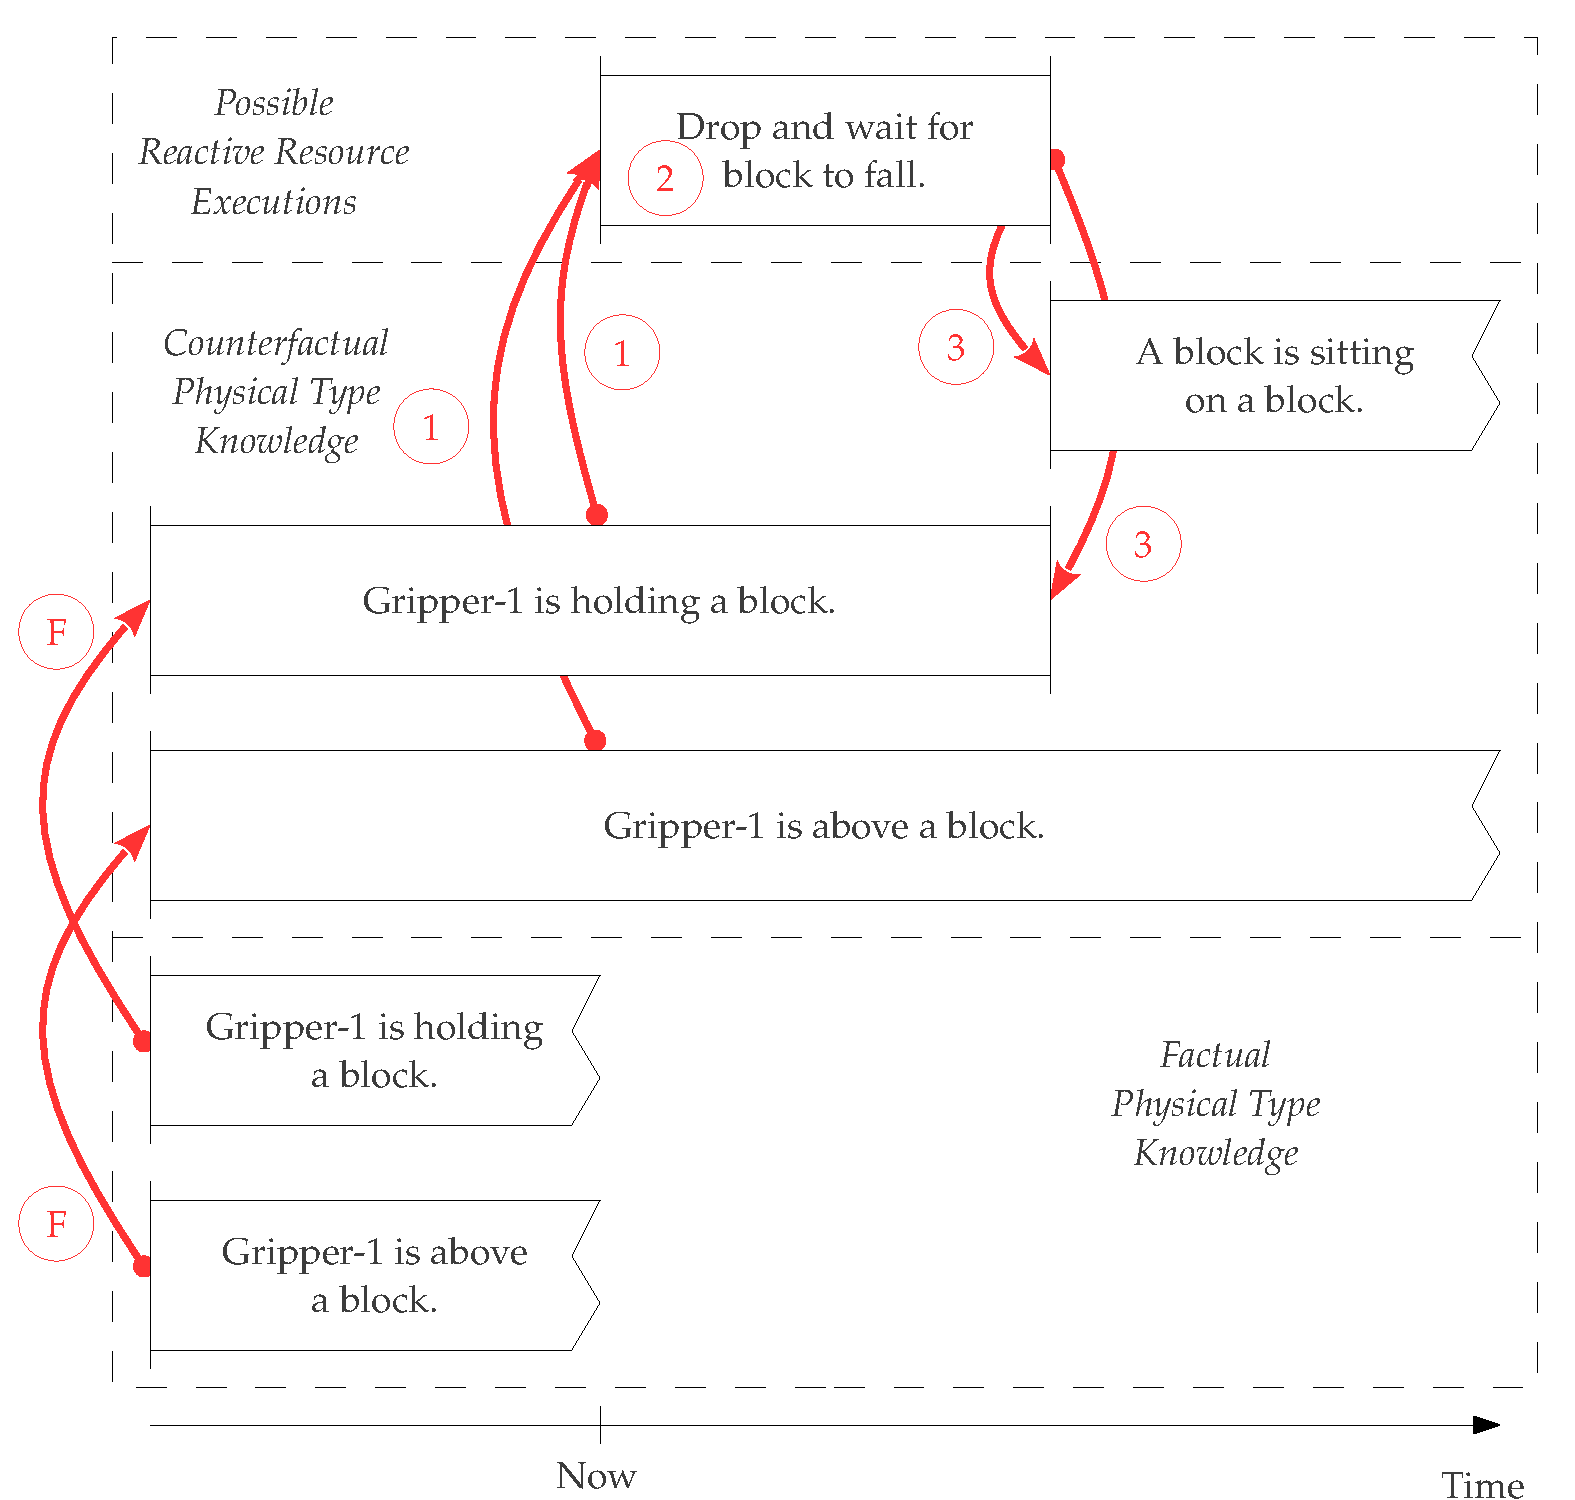
\includegraphics[width=12cm]{gfx/inference_of_physical_knowledge}
\caption[Inference of counterfactual physical type knowledge from
  factual physical type knowledge.]{Inference of counterfactual
  physical type knowledge from factual physical type knowledge.
  Rectangular boxes represent events over time.  Some events have a
  jagged right edge to indicate that this event has no ending time.
  Curved arrows represent different dependency relationships: (F)
  factual, (1) precondition, (2) potential resource execution, and (3)
  hypothetical change.  Preconditions, potential resource activations,
  and hypothetical changes form the three possibly unsupported parts
  of a dependency.  Factual dependencies cannot lose support because
  they are derived directly from factual events.}
\label{figure:inference_of_physical_knowledge}
\end{figure}
